\documentclass[12pt]{article}
\usepackage{amsmath, graphicx, caption}
\usepackage{amsthm}
\usepackage{amsfonts, xcolor, physics, listings,verbatim,float}
\usepackage{amssymb}
\usepackage{mathrsfs}
\usepackage[T1]{fontenc} % for \symbol{92} 
\usepackage{comment, subfig, hyperref}


\addtolength{\oddsidemargin}{-1in}
\addtolength{\evensidemargin}{-1in}
\addtolength{\textwidth}{1.75in}
\addtolength{\topmargin}{-1in}
\addtolength{\textheight}{1.75in}
\newcommand{\contra}{$\rightarrow\leftarrow$}
\newcommand{\tb}{  \textbackslash  }
\newcommand{\bj}{\ \Longleftrightarrow \ }

%bailey meche
\begin{document}
%bailey meche
	\begin{center}
		ECMA 30150: Perspectives on Computational Modeling for Economics\\
        Problem Set 3 \\
		Due Date: January 28th, 2025 \\
        Bailey Meche
	\end{center}

\section*{Instructions}
You are encouraged to work and discuss in groups, but you must submit your work individually. Answers must be legibly hand-written or typed. All assignments are due electronically on Canvas, and you must attach your code. Assignments are due at \textbf{12:30 PM}. \textbf{Late problem sets will not be accepted.}

\section*{Problem 1: The Neoclassical Growth Model I (100 points)}
A Central planner uses a Bellman equation to state the problem as:
\[
v(k) = \max_{c,k'} \left[ u(c) + \beta v(k') \right]
\]
subject to:
\[
k' + c = F(k, 1) + (1 - \delta)k
\]

\subsection*{(a) (30 points)}
Assume \( u(c) = \ln(c) \), \( \delta = 1 \), and \( F(k, 1) = k^\alpha \). Use the guess and verify method to find the value function and the associated policy functions.

\subsubsection*{Solution}

Substituting the constraint into the Bellman equation and making the guess: 
\[
v(k) = \max_{k'} \left[ \ln(k^\alpha -k') + \beta v(k') \right] = A+B\ln(k).
\]
We substitute $v(k') = A+B\ln(k')$:
\begin{align*}
    A+B\ln(k) &= \max_{k'} \left[ \ln(k^\alpha -k') + \beta (A+B\ln(k')) \right] 
    \\ A(1-\beta) + B\ln(k) &= \max_{k'} \left[ \ln(k^\alpha -k') + \beta B\ln(k') \right] 
\end{align*}
Taking the FOC of the RHS:
\begin{align*}
   \frac{\partial}{\partial k'}\left[ \ln(k^\alpha -k') + \beta B\ln(k') \right]&=0
   \\ k' &= \frac{\beta B}{1 + \beta B}k^\alpha
\end{align*}
Substituting back into Bellman to solve for $A,B$,
\[ B = \frac{\alpha}{1-\beta}; \quad A = \frac{\ln(1-\beta B)}{1-\beta}.\]
Hence, the value function is
\[
v(k) = \frac{\ln(1 - \beta \frac{\alpha}{1 - \beta})}{1 - \beta} + \frac{\alpha}{1 - \beta} \ln(k).
\]
and the policy functions are:
\[
k' = \frac{\beta \alpha}{1 + \beta \alpha} k^\alpha,
\]
\[
c = k^\alpha - \frac{\beta \alpha}{1 + \beta \alpha} k^\alpha = \frac{k^\alpha}{1 + \beta \alpha}.
\]

\bigskip

\subsection*{(b) (70 points)}
Now use the following functional forms and parameters:
\[
u(c) = \frac{c^{1-\sigma}}{1-\sigma}, \quad \sigma = 2, \quad F(k, 1) = k^\alpha, \quad \alpha = 0.4, \quad \delta = 0.03, \quad \beta = 0.95
\]
Assume a range of approximation \( [k_{\min} = 0.1\bar{k}, k_{\max} = 1.2\bar{k}] \), where \( \bar{k} \) is the steady-state stock of capital. Use the Orthogonal Collocation method to find (an approximation of) the policy function for the stock of capital \( k' \equiv \hat{g}(k, a) \). Start with the approximation under \( \sigma = \delta = 1 \), where the solution is known. Use at least \( n = 7 \) nodes for approximation.

\subsubsection*{Solution}

%\subsection*{1. Parameters and Steady-State Capital}
The steady-state capital stock $\bar{k}$ is computed as:
\[
\bar{k} = \left( \frac{\alpha \beta}{1 - \beta (1 - \delta)} \right)^{\frac{1}{1 - \alpha}} = \left( \alpha \beta \right)^{\frac{1}{1 - \alpha}},
\]

%\subsection*{2. Chebyshev Nodes and Basis Functions}
The Chebyshev nodes $z_\ell$ in $[-1, 1]$ are given by:
\[
z_\ell = -\cos\left(\frac{2\ell - 1}{2n} \pi\right), \quad \ell = 1, 2, \dots, 7.
\]

These are mapped to the interval $[k_{\min}, k_{\max}]$:
\[
k_\ell = \frac{(z_\ell + 1)(k_{\max} - k_{\min})}{2} + k_{\min}.
\]

The Chebyshev basis functions are defined as:
\[
T_i(\xi) = \cos\left(i \cdot \arccos(\xi)\right), \quad i = 0, 1, \dots, n,
\]
where:
\[
\xi(k) = \frac{2(k - k_{\min})}{k_{\max} - k_{\min}} - 1.
\]

%\subsection*{3. Policy Function Approximation}
The policy function $\hat{g}(k; \mathbf{a})$ is approximated as:
\[
\hat{g}(k; \mathbf{a}) = \sum_{i=0}^{n} a_i T_i(\xi(k)),
\]
where $\mathbf{a} = [a_0, a_1, \dots, a_n]^\top$ are the coefficients.
%\subsection*{4. Residual Function for the Euler Equation}
The Euler equation is:
\[
u'(f(k) - \hat{g}(k; \mathbf{a})) = \beta u'(f(\hat{g}(k; \mathbf{a})) - \hat{g}(\hat{g}(k; \mathbf{a}); \mathbf{a})) \cdot f'(\hat{g}(k; \mathbf{a})),
\]
where:
\begin{align*}
f(k) &= k^\alpha + (1 - \delta)k, \\
f'(k) &= \alpha k^{\alpha - 1} + 1 - \delta, \\
u'(c) &= c^{-\sigma}.
\end{align*}

The residual function $R(k, \mathbf{a})$ is enforced to be zero at the $n+1$ collocation nodes:
\[
R(k_\ell, \mathbf{a}) = 0, \quad \ell = 1, 2, \dots, n+1.
\]
Using a numerical solver (e.g., \texttt{fsolve}), the coefficients $\mathbf{a}$ are determined.
%\subsection*{6. Policy Function Evaluation on a Fine Grid}
On a fine grid $k \in [k_{\min}, k_{\max}]$, the policy function is evaluated as:
\[
\hat{g}(k; \mathbf{a}) = \mathbf{T}(k) \cdot \mathbf{a},
\]
where $\mathbf{T}(k)$ is the matrix of Chebyshev polynomials evaluated at the grid points.
%\subsection*{7. Results Visualization}
The approximated policy function is plotted alongside the 45-degree line for comparison:
\[
\text{Plot: } k_{t+1} = \hat{g}(k_t; \mathbf{a}) \text{ vs. } k_{t+1} = k_t.
\]
See figure \eqref{fig:1b}.

\begin{figure}[H]
    \centering
        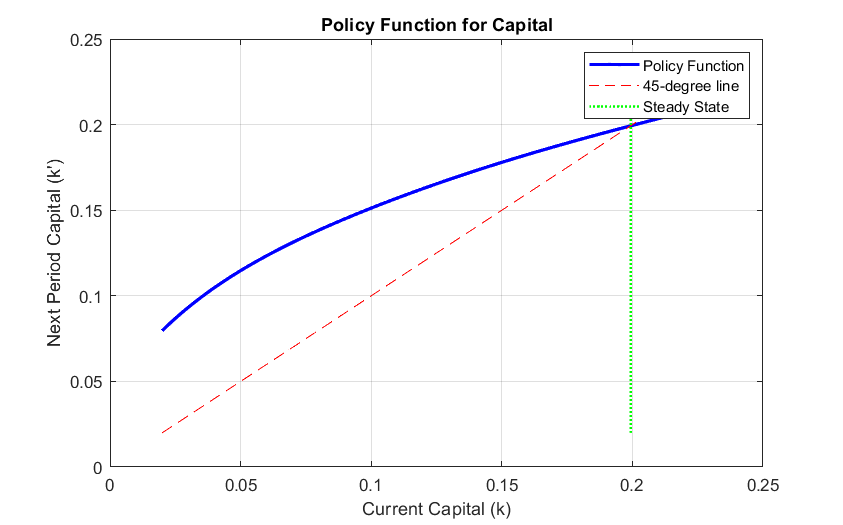
\includegraphics[width=\textwidth]{pset3_q1b.png}
        \caption{Orthogonal Collocation Approximation of $k'$ for Problem 1 (b).}
        \label{fig:1b}
\end{figure}


\iffalse 
\subsection{deleted}
%\begin{enumerate}
%\item \textbf{Set up the Euler equation.}  
From first-order conditions,
\[
u'\bigl(c_t\bigr)
\;=\;
\beta\,u'\bigl(c_{t+1}\bigr)\,\bigl[F'(k_{t+1}) + 1-\delta\bigr],
\]
where $c_t = k_t^\alpha + (1-\delta)\,k_t - k_{t+1}$.
For $\sigma=2$, 
\[
u'(c) \;=\; c^{-2},
\]
so the Euler equation becomes
\[
c_t^{-2}
\;=\;
\beta\,c_{t+1}^{-2}\,\Bigl[\alpha\,k_{t+1}^{\,\alpha-1} + 1-\delta\Bigr].
\]

%\item \textbf{Choose an approximation form.}  
We posit 
\[
k_{t+1} \;=\; g(k_t;\mathbf{a})
\]
where $\mathbf{a}=(a_0,a_1,\dots,a_n)$ are unknown coefficients.  A convenient choice is a \emph{Chebyshev polynomial expansion}:
\[
k_{t+1} \;=\; \hat g(k_t;\mathbf{a})
\;=\;
\sum_{j=0}^n
a_j\,T_j\!\Bigl(\ell(k_t)\Bigr),
\]
where $T_j$ is the $j$-th Chebyshev polynomial and $\ell(\cdot)$ maps $k_t$ from the interval $[\,k_{\min},k_{\max}\,]$ to $[-1,1]$.

%\item \textbf{Collocation nodes.}  
Select $n+1$ \emph{Chebyshev nodes} 
\[
k_i
\;\in\;
[k_{\min},\,k_{\max}], 
\qquad i=0,\dots,n,
\]
(usually scaled from the usual Chebyshev points in $[-1,1]$).  We take $n=7$ (at least).

%\textbf{Form the residual and enforce $=0$ at each node.}  
Define 
\[
R\bigl(k;\mathbf{a}\bigr)
\;=\;
u'\!\Bigl(\underbrace{k^\alpha+(1-\delta)\,k - g(k;\mathbf{a})}_{c(k;\mathbf{a})}\Bigr)
\;-\;
\beta\;u'\!\Bigl(\underbrace{(g(k;\mathbf{a}))^\alpha + (1-\delta)\,g(k;\mathbf{a}) - g\bigl(g(k;\mathbf{a});\mathbf{a}\bigr)}_{c\bigl(g(k)\bigr)}\Bigr)
\;\bigl[\alpha\,\bigl(g(k;\mathbf{a})\bigr)^{\alpha-1} + (1-\delta)\bigr].
\]
At each node $k_i$, impose $R(k_i;\mathbf{a})=0$.  This gives $n+1$ equations in the $n+1$ unknowns $\mathbf{a}$.

%\item \textbf{Solve the nonlinear system.} 
se a root-finder (e.g.\ Newton's method) to solve $R(k_i;\mathbf{a})=0$ for all $i=0,\dots,n$.

% \textbf{Result.}  
The converged coefficients $\widehat{\mathbf{a}}$ define the approximate policy:
\[
k_{t+1} \;\approx\; g(k_t;\widehat{\mathbf{a}}).
\]
%\end{enumerate}

A standard trick is to begin with a simpler case whose solution is known (e.g.\ $\sigma=1$ or $\delta=1$) to get a good initial guess for $\mathbf{a}$.  This improves convergence.  In practice, one iterates until the residual is acceptably small.

\fi




\section*{Problem 2: The Neoclassical Growth Model II (110 points)}
A Central planner uses a Bellman equation to state the problem as:
\[
v(k) = \max_{c,k'} \left[ u(c) + \beta v(k') \right]
\]
subject to:
\[
k' + c = F(k, 1) + (1 - \delta)k
\]
Use the following functional forms and parameters:
\[
u(c) = \frac{c^{1-\sigma}}{1-\sigma}, \quad \sigma = 2, \quad F(k, 1) = k^\alpha, \quad \alpha = 0.36, \quad \delta = 0.025, \quad \beta = 0.95
\]

\subsection*{(a) (10 points)}
Find the Euler equation.

\subsubsection*{Solution}
We have:
\[
\max_{\{c_t,k_{t+1}\}}\;\sum_{t=0}^\infty \beta^t u \bigl(c_t\bigr),
\quad\text{subject to}\quad
k_{t+1} + c_t \;=\;k_t^\alpha + (1-\delta)\,k_t,
\]
where
\[
u(c)
\;=\;
\frac{c^{1-\sigma}}{\,1-\sigma\,},
\quad
\sigma=2,\quad
\alpha=0.36,\quad
\delta=0.025,\quad
\beta=0.95.
\]

%\subsection*{(a) \quad The Euler Equation}

From the planner's FOC, we have
\[
u'(c_t)
\;=\;
\beta\;u'\!\bigl(c_{t+1}\bigr)\,
\Bigl[\alpha\,k_{t+1}^{\,\alpha-1} + (1-\delta)\Bigr],
\]
with
\[
c_t \;=\; k_t^\alpha + (1-\delta)\,k_t \;-\; k_{t+1}.
\]
Since $\sigma=2$, $u'(c)=c^{-2}$.  Hence, we have the Euler equation
\[
c_t^{-2}
\;=\;
\beta\,c_{t+1}^{-2}\;\bigl[\alpha\,k_{t+1}^{\,\alpha-1} + 1-\delta\bigr].
\]
%his is the required Euler equation.


\subsection*{(b) (10 points)}
Find the steady state of the model.

\subsubsection*{Solution}
In steady state, $k_{t+1}=k_t=\hat{k}$ and $c_t=\bar{c}$ are constant.  Then the feasibility condition implies
\[
\bar{c} \;=\; (\hat{k})^\alpha + (1-\delta)\,\hat{k} - \hat{k}.
\]
But more directly we use the Euler equation at steady state:
\[
(\bar{c})^{-2}
\;=\;
\beta\,(\bar{c})^{-2}\,\Bigl[\alpha\,(\bar{k})^{\alpha-1} + 1-\delta\Bigr].
\]
Cancelling $(\bar{c})^{-2}$ from both sides gives
\[
1
\;=\;
\beta\,\bigl[\alpha\,(\bar{k})^{\alpha-1} + (1-\delta)\bigr].
\]
Hence
\[
\alpha\,(\bar{k})^{\,\alpha-1} + (1-\delta)
\;=\;
\frac{1}{\,\beta\,}.
\]
One solves for $\bar{k}$:
\[
\alpha\,(\bar{k})^{\,\alpha-1}
\;=\;
\frac{1}{\,\beta\,} - (1-\delta),
\]
then $\bar{c}=\bar{k}^{\alpha}+(1-\delta)\,\bar{k}-\bar{k}$.  


\subsection*{(c) (20 points)}
Find a linear approximation around the steady state of both the Euler equation and the feasibility constraint. Write the system in the form:
\[
y_{t+1} = Ay_t
\]
\subsubsection*{Solution}
%\subsection*{(c) \quad Linear Approximation Around the Steady State}

Define small deviations:
\[
\hat{k}_t 
\;=\;
k_t - \bar{k},
\quad
\hat{c}_t
\;=\;
c_t - \bar{c}.
\]
We wish to linearize both the feasibility condition and the Euler equation to get a system of the form
\[
\begin{pmatrix}
\hat{k}_{t+1} \\[6pt]
\hat{c}_{t+1}
\end{pmatrix}
\;=\;
A\,
\begin{pmatrix}
\hat{k}_t \\[4pt]
\hat{c}_t
\end{pmatrix}.
\]
%\paragraph{1. Linearizing the feasibility constraint.}
\[
k_{t+1} + c_t = k_t^\alpha + (1-\delta)\,k_t.
\]
We have the following for the production and utility functions: 
\begin{align*}
    f'(k) &= \alpha k^{\alpha-1} +1-\delta & u'(c) = c^{-\sigma}
    \\ f''(k)&= \alpha(\alpha-1)k^{\alpha-2} & u''(c)=-\sigma c^{-(1+\delta)}
\end{align*}
Plugging these in, we have the linearized system 
\[
\begin{pmatrix}
\hat{k}_{t+1}\\[6pt]
\hat{c}_{t+1}
\end{pmatrix}
=
\begin{pmatrix}
\frac{1}{\beta} & -1 \\ \frac{c^{-\sigma} \alpha(\alpha-1)k^{\alpha-2} }{\sigma c^{-(1+\delta)}} & 1+ \frac{\beta c^{-\sigma} \alpha(\alpha-1)k^{\alpha-2}}{\sigma c^{-(1+\delta)}}
\end{pmatrix}
\begin{pmatrix}
\hat{k}_t\\[4pt]
\hat{c}_t
\end{pmatrix}
\]
from the results in the notes. 


\subsection*{Part (d) (10 points)}
Use Matlab (or any other software) to find the eigenvectors and eigenvalues of \( A \). Check that eigenvalue \( \lambda_1 \) is smaller than one and eigenvalue \( \lambda_2 \) is higher than one.

\subsubsection*{Solution}

\[ \lambda_1 = 0.9557; \quad \lambda_2 =  1.1015, \]        
\[  v_2  = \begin{bmatrix}0.9953 \\
      0.0965\end{bmatrix}; \quad v_2  = \begin{bmatrix}-0.0488 \\0.9988\end{bmatrix}.\]
   
\subsection*{Part (e) (30 points)}
Find the policy functions:
\[
c_t - \bar{c} = -\frac{\tilde{v}_{21}}{\tilde{v}_{22}} (k_t - \bar{k}),
\]
\[
k_{t+1} - \bar{k} = \lambda_1 (k_t - \bar{k}),
\]
where \( \tilde{v}_{ij} \) is the position \((i, j)\) of the matrix \( V^{-1} \). Simulate the transition starting at 10\% of steady-state capital stock.
\subsubsection*{Solution}
See figure \eqref{fig:2e}.

\begin{figure}[H]
    \centering
        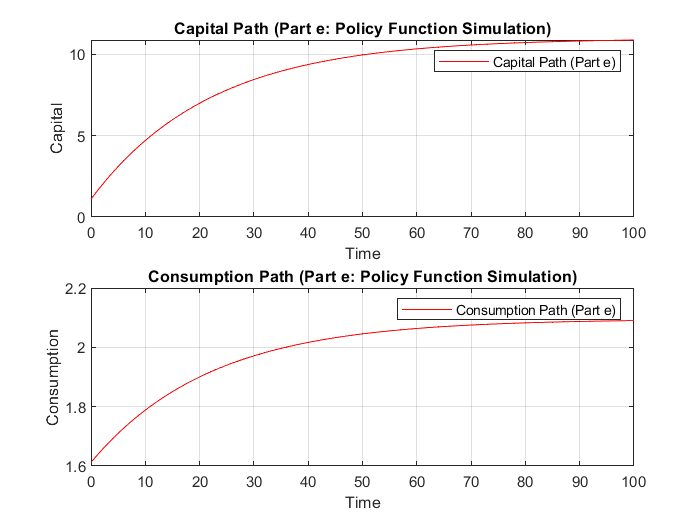
\includegraphics[width=\textwidth]{pset3_2e.png}
        \caption{Simulate of transition dynamics starting at 10\% of steady-state capital stock for Problem 2 (e).}
        \label{fig:2e}
\end{figure}

\subsection*{Part (f) (15 points)}
Use Dynare to find the time paths of both capital and consumption. Compare these paths to the ones derived in Part (e).
\subsubsection*{Solution}
See figure \eqref{fig:2f}.

\begin{figure}[H]
    \centering
        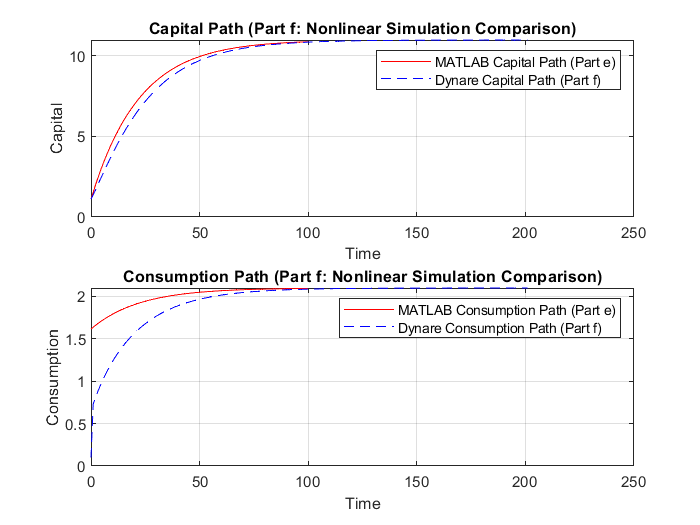
\includegraphics[width=\textwidth]{pset3_2f.png}
        \caption{Dynare Time Paths of both Capital and Consumption for Problem 2 (f).}
        \label{fig:2f}
\end{figure}

\subsection*{Part (g) (15 points)}
Use Dynare to find the time paths of capital and consumption under a linear approximation. Compare these paths to the ones derived in Part (e).
\subsubsection*{Solution}
See figure \eqref{fig:2g}.

\begin{figure}[H]
    \centering
        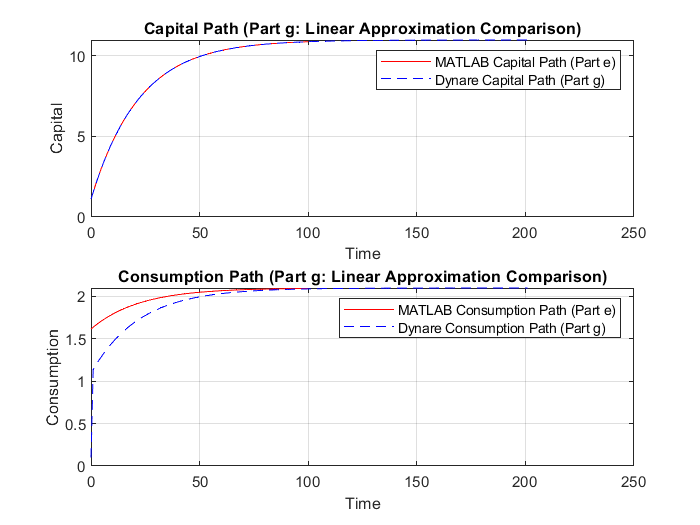
\includegraphics[width=\textwidth]{pset3_2g.png}
        \caption{Dynare Time Paths of both Capital and Consumption (Linear Approximation) for Problem 2 (g).}
        \label{fig:2g}
\end{figure}

\section*{Problem 3: The Neoclassical Growth Model with Variable Labor Supply (80 points)}
A Central planner uses a Bellman equation to state the problem as:
\[
v(k) = \max_{c, \ell, k'} \left[ u(c, \ell) + \beta v(k') \right]
\]
subject to:
\[
k' + c = F(k, \ell) + (1 - \delta)k
\]
Use the following functional forms and parameters:
\[
u(c, \ell) = \ln(c) + \gamma(1 - \ell), \quad F(k, \ell) = k^\alpha \ell^{1-\alpha}, \quad \alpha = 0.36, \quad \delta = 0.025, \quad \beta = 0.95
\]
Here, \( \ell \) is the amount of working time, normalized to unity. \( \gamma > 0 \) measures the disutility of work. Note that \( \gamma \) is not given and must be calibrated.

\subsection*{(a) (20 points)}
Find the Euler equation and the relevant first-order conditions (FOCs) using a Lagrangian. Derive three equations that form a dynamic system for \( k_t, c_t, \ell_t \).

\subsubsection*{Solution}
The Lagrange is given by 
\[ \mathcal{L} = \sum_{t=0}^\infty \beta^t \left[ \ln(c_t) + \gamma(1- l_t) + \lambda_t \left( k_t^\alpha l_t^{1-\alpha} + (1-\delta) k_t - k_{t+1} - c_t\right) \right]\]
with Lagrange multipliers $\lambda_t.$
FOCs are given by 
\begin{align*}
    \frac{\partial \mathcal{L}}{\partial c_t } &= \beta^t \left[ \frac{1}{c_t} - \lambda_t \right] =0 & \implies & \lambda_t = \frac{1}{c_t} 
    \\ \frac{\partial \mathcal{L}}{\partial l_t } &= \beta^t \left[ -\gamma + \lambda_t (1-\alpha)k_t^\alpha l_t^{-\alpha}\right] =0 &\implies& \lambda_t = \frac{\gamma l_t^{\alpha}}{ (1-\alpha)k_t^\alpha }
    %%%%%%%%%%%%%%%%%
    \\ &&\implies& \frac{1}{c_t} = \frac{\gamma l_t^{\alpha}}{ (1-\alpha)k_t^\alpha }
    \\ &&\implies& c_t = \frac{ (1-\alpha)k_t^\alpha }{\gamma l_t^{\alpha}}
    \\ \frac{\partial \mathcal{L}}{\partial k_{t+1} } &= \beta^t(-\lambda_t) + \beta^{t+1} \left[ \frac{1}{c_{t+1}} ( \alpha k_{t+1}^{\alpha-1} l_{t+1}^{1-\alpha} +1-\delta)\right] &\implies& c_t = \frac{c_{t+1} }{ \beta( \alpha k_{t+1}^{\alpha-1} l_{t+1}^{1-\alpha} +1-\delta)}
\end{align*}

Hence we have our Euler equation 
\begin{equation}\label{Euler}
    c_t = \frac{c_{t+1} }{ \beta( \alpha k_{t+1}^{\alpha-1} l_{t+1}^{1-\alpha} +1-\delta)}
\end{equation}
subject to the labor-supply condition
\begin{equation}\label{labor-supply}
    c_t = \frac{ (1-\alpha)k_t^\alpha }{\gamma l_t^{\alpha}}
\end{equation}
and the resource constraint
\begin{equation}\label{resource}
    c_t + k_{t+1} = k_t^\alpha \ell_t^{1-\alpha}  + (1-\delta) k_t.
\end{equation}


\subsection*{(b) (20 points)}
In the steady state, under some parameterization, the system derived in Part (a) gives three equations for the unknowns \( \bar{k}, \bar{c}, \bar{\ell} \) (steady-state values). Since \( \gamma \) is not provided, set \( \bar{\ell} = \frac{1}{3} \) and use the system to solve for \( \bar{k}, \bar{c}, \gamma \).

\subsubsection*{Solution}
In steady state, $k_t = \bar{k} , c_t = \bar{c}, l_t = \bar{l}$. Hence, from \eqref{Euler}:
\begin{align}
     \bar{c} &= \frac{\bar{c} }{ \beta( \alpha \bar{k}^{\alpha-1} \bar{l}^{1-\alpha} +1-\delta)} \notag
     \\  \alpha \bar{k}^{\alpha-1} \bar{l}^{1-\alpha} +1-\delta &=  \frac{1}{\beta}\notag
     %%%%%%%%%%%%
     \\  \bar{k} &=  \left(\frac{\frac{1}{\beta} -1+\delta }{\alpha  \bar{l}^{1-\alpha}}\right)^{\frac{1}{1-\alpha}}\label{k_ss}
     %= \left(\frac{ \bar{l}^{\alpha-1}}{\beta\alpha\ }+\frac{\delta-1}{\alpha\ \bar{l}^{\alpha-1}\ }\right)^{1-\alpha}
\end{align}
which is fully calculable since $ \bar{\ell} = \frac{1}{3}.$ From \eqref{labor-supply}:
\begin{align}
    \bar{c} = \frac{(1-\alpha)\bar{k}^\alpha }{\gamma \bar{l}^{\alpha}} \label{ss_labor-supply}
\end{align}
From \eqref{resource}:
\begin{align}
    \bar{c} + \bar{k} &= \bar{k}^\alpha \bar{l}^{1-\alpha}  + (1-\delta) \bar{k}\notag
    \\ \bar{c} &=  \bar{k}^\alpha \bar{l}^{1-\alpha}  -\delta \bar{k} \label{c_ss}
\end{align}
which is fully calculable. Since we have \eqref{k_ss} and \eqref{c_ss}, we have
\begin{align}
     \gamma= \frac{(1-\alpha)\bar{k}^\alpha }{ \bar{c}\bar{l}^{\alpha}} \label{gamma}
\end{align}
from \eqref{ss_labor-supply}. Therefore, $k_t, c_t, \ell_t $ are given by \eqref{k_ss},\eqref{c_ss}, and \eqref{gamma} respectively.

\subsection*{Part (c) (20 points)}
Use Dynare to find the time paths of capital, consumption, and labor. Simulate the transition starting at 10\% of steady-state capital stock.

\subsubsection*{Solution}
See figure \eqref{fig:3c}.

\begin{figure}[H]
    \centering
        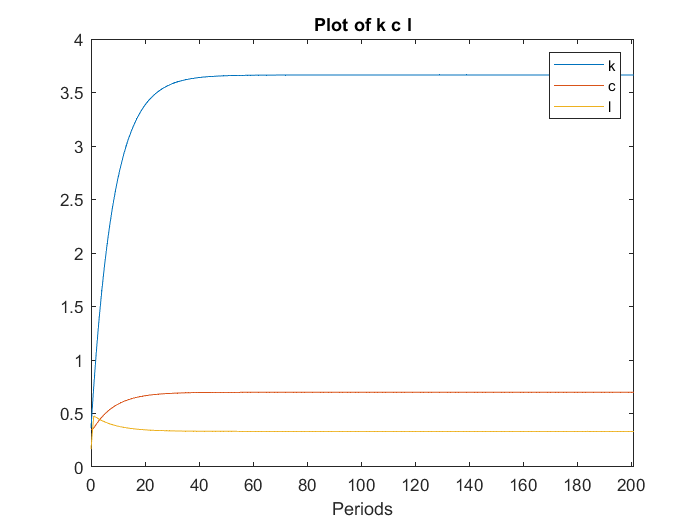
\includegraphics[width=\textwidth]{pset3_3c.png}
        \caption{Simulate the time paths of capital, consumption, and labor starting at 10\% of steady-state capital stock for Problem 3 (c).}
        \label{fig:3c}
\end{figure}
    
\subsection*{Part (d) (20 points)}
Use Dynare to find the time paths of capital, consumption, and labor under a linear approximation. Compare these paths to the ones derived in Part (c). Simulate the transition starting at 10\% of steady-state capital stock.

\subsubsection*{Solution}
See the figures below. 

\begin{figure}[H]
    \centering
        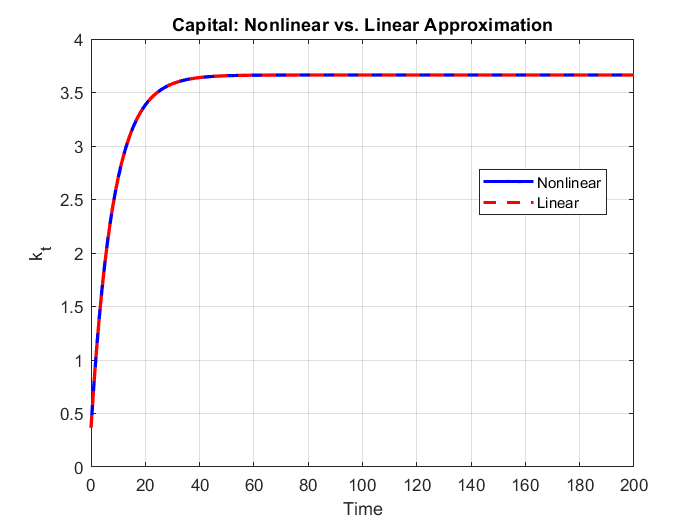
\includegraphics[width=\textwidth]{pset3_3d_fig1.png}
       
\end{figure}
\begin{figure}[H]
    \centering
        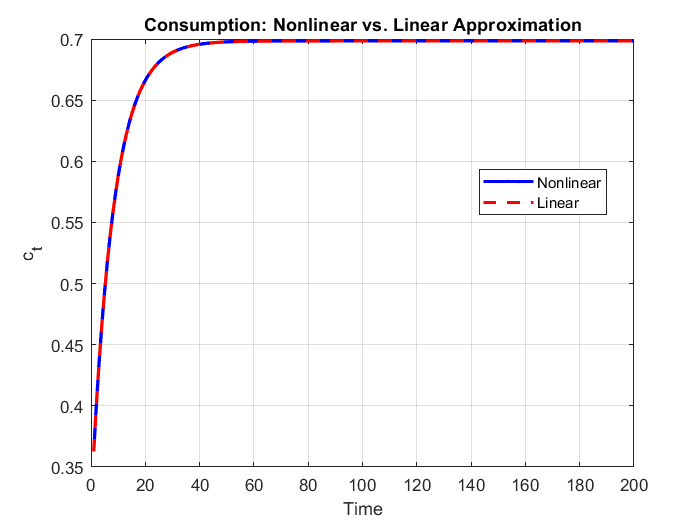
\includegraphics[width=\textwidth]{pset3_3d_fig2.png}
\end{figure}
\begin{figure}[H]
    \centering
        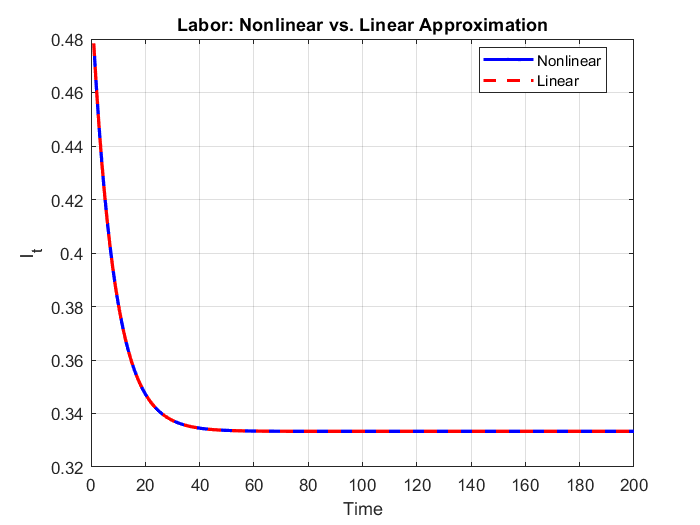
\includegraphics[width=\textwidth]{pset3_3d_fig3.png}

\end{figure}
\end{document}